\section{Sampling}
It is often needed to sample from a joint distribution, of the form $P(y_1, \cdots, y_n)$ or $P(\mathbf x = x_1, \cdots, x_n)$ or $P(x_1, \cdots, x_r | x_{r+1} = E_{r+1}, \cdots, x_n = E_n)$. Some scenarios might be
\begin{enumerate}
	\item Solving an intractable inference during training
	\item Showing a diverse set of outputs instead of just the most likely value
	\item Calculating the expected value of some arbitrary function $f(\mathbf x)$ under distribution $P(\mathbf x)$.
\end{enumerate}
\subsection{Motivation}
\begin{itemize}
	\item[$\diamond$] Say we have a deep language model, we might want to generate sample sentences, questions or expected distribution of first word for sentences ending with '?'.
	\item [$\diamond$] We can use VAEs for missing value imputation. This can be done by fixing values of some of the outputs, and generate most likely values of others.  
\end{itemize}
We had seen in VAEs how to approximate the expected value of a function with sampling. Say we have a function $f(\mathbf x): \mathcal{X} \to \mathbb{R}$ and we want $\mathbb{E}_{P(\mathbf x)}[f(\mathbf x)] = \sum_{\mathbf x \in \mathcal X} f(\mathbf x) P(\mathbf x)$. In case of continuous $\mathbf x$, we can take the integral. Our space $\mathcal X$ is very large, and we cannot compute the integral exactly in closed form. Hence we want to sample and approximate the expectation. Say we have samples $\mathbf x^1, \cdots, \mathbf x^M \sim P(\mathbf x)$, we write
\begin{equation}
	\mathbb{E}_{P(\mathbf x)}[f(\mathbf x)] = \sum_{\mathbf x \in \mathcal X} f(\mathbf x) P(\mathbf x) \approx \dfrac{1}{M} \sum_{i=1}^M f(\mathbf x^i)
\end{equation}
As $M \to \infty$, this approximation matches exact expected value.
\subsection{Sampling scalar distributions}
Let $p(x)$ be a distribution, and we want to draw samples $x^1, \cdots, x^M$. Say we can sample $u$ from $U(0,1)$ (uniform distribution). Let $F(x)$ be the CDF of $p(x)$. \\
\noindent For $i=1, \cdots, M$ \\
$\triangleright$ Sample $u_i \sim U(0,1)$ \\
$\triangleright$ Find $x_i = F^{-1}(u)$ \\
\noindent Now, say we a multinomial distribution. Say $x$ is discrete and $\in \{1, \cdots, m\}$. We have $p(x) \sim Mult(p_1, \cdots, p_m)$, $u_i \sim U(0,1)$, and if $u_i$ is between $\sum_{j=0}^{k-1} p_j$ and $\sum_{j=0}^{k} p_j$, choose $k$. 

Now, as $M \to \infty$, the fraction of times we encounter a sample in the interval $[x, x+\Delta)$ would be proportional to the true probability of that in the interval in $p(x)$, i.e $F(x+\Delta) - F(x)$.
\subsection{Sampling multivariate distributions}
One option to sample from multivariate distributions is to factorize the distribution as a Bayesian Network, and perform \textit{forward sampling}. Such a method is used in autoregressive language models. Assume
\[P(\mathbf x) = \prod_{j=1}^n P(x_j | \text{Pa}(x_j))\]
Now, $y_j \sim P(y_j | y_1, \cdots, y_{j-1}, \mathbf x)  = P(y_j | s_j, \mathbf x)$. The $s_j$ is called the state in RNNs, and the calculation of probability is called softmax. \\
\begin{algorithm}[H]\label{alg:s-fs}
	\DontPrintSemicolon
	$x_1, \cdots, x_n \longleftarrow$ topologically sorted according to BN \;
	\For{$i = 1$ to $M$}{
		$\xi^i = [0, \cdots, 0]$\;
		\For{$j=1$ to $n$}{
			$\xi^i_j \sim P(x_j | \xi^i_{\text{Pa}(x_j)})$\;
		}
	}
	\Return{$\xi^1, \cdots, \xi^M$}
	\caption{Forward Sampling Algorithm}
\end{algorithm}
\begin{marginfigure}
	\centering
	\begin{tikzpicture}[main/.style = {draw, circle}] 
		\node[main] (a) {$x_1$}; 
		\node[main] (b) [right of=a] {$x_2$};
		\node[main] (c) [below = of $(a)!0.5!(b)$] {$x_3$};
		\node[main] (d) [below right of=c] {$x_4$};
		\node[main] (e) [below left of=d] {$x_5$};
		\draw[->] (a) -- (c);
		\draw[->] (b) -- (c);
		\draw[->] (c) -- (d);
		\draw[->] (d) -- (e);
		\draw[->] (c) -- (e);
	\end{tikzpicture}
	\caption{BN Example}
	\label{fig:s-exmp-1}
\end{marginfigure}
\begin{exmp}
Consider the BN shown in Figure \ref{fig:s-exmp-1}. We start with $x_1$ as it has no parents, and we want to get $\xi^1$. 
\begin{enumerate}
	\item $x_1 \sim P(x_1)$. Say $x_i$ were binary, and we get $\xi_1^1 = 0$.
	\item $x_2 \sim P(x_2)$. Say we get $\xi^1_2 = 1$. 
	\item $x_3 \sim P(x_3 | x_1 = 0, x_2 = 1)$. Say we get $\xi^1_3 = 1$.
\end{enumerate}
We can proceed similarly and get our sample $\xi^1$.
\end{exmp}
There are drawbacks of forward sampling - mainly being it will not be consistent when we have conditions imposed. Say we want to get the probability of $x_1$ being `what' when ! is the last token. Forward sampling would have most of the sampled sentences wasted since they don't end with `!'. Another example could be when we want to complete a missing attribute in a VAE network for object generation and in this case forward sampling wouldn't match the given values most of the time. \\
In such cases we use \textbf{importance sampling}. It is useful when it is hard to sample from $P(\mathbf x)$ or to lower the error in computation of the expected value of the function, i.e $\mathbb{E}_{P(\mathbf x)} [f(\mathbf x)]$, where $f(\mathbf x)$ has zeros at a large number of $\mathbf x$. Importance sampling samples from the important regions. \\
In importance sampling, we get to choose $Q(\mathbf x)$, called the proposal distribution, from which it is easy to generate samples. Designing such a $Q(\mathbf x)$ is problem-dependent. For example, in a language modeling task, $Q(\mathbf x)$ is the reverse language model. \\
Say we generate $S_Q = \{\mathbf x^1, \cdots, \mathbf x^M\}$ from $Q(\mathbf x)$. In general $\forall$ functions, $\mathbb{E}_{Q(\mathbf x)}[f(\mathbf x)] \neq \mathbb{E}_{P(\mathbf x)}[f(\mathbf x)] $. We use the following trick
\begin{align*}
	\mathbb{E}_{P(\mathbf x)}[f(\mathbf x)] &= \sum_{\mathbf x} f(\mathbf x)P(\mathbf x) \\
	&= \sum_{\mathbf x} Q(\mathbf x) \dfrac{P(\mathbf x)}{Q(\mathbf x)}f(\mathbf x) \qquad\text{let } W(\mathbf x) = \dfrac{P(\mathbf x)}{Q(\mathbf x)}\\
\mu_P(S_Q)	&= \dfrac{1}{M} \sum_{i=1}^M \big[ f(\mathbf x^i) W(\mathbf x^i) \big] \qquad\text{(Importance weighted estimate)}
\end{align*}
\begin{algorithm}[H]\label{alg:s-is}
	\DontPrintSemicolon
	\textbf{Given:} $M, Q(\mathbf x), P(\mathbf x)$\;
	\For{$i = 1$ to $M$}{
		$\xi^i \longleftarrow$ Sample from $Q(\mathbf x)$\;
		$W^i \longleftarrow \dfrac{P(\xi^i)}{Q(\xi^i)}$
	}
	\Return{$(\xi^1, W^1), \cdots, (\xi^M, W^M)$}
	\caption{Importance Sampling Algorithm}
\end{algorithm}
The user can decide what to do with the samples, for example
\begin{equation}
	\mathbb{E}_{P(\mathbf x)}[f(\mathbf x)] = \dfrac{1}{M} \sum_{i=1}^M f(\xi^i) W^i
\end{equation}
The limitations for the above algorithm is that it is not applicable for $P(\mathbf x)$ where we have an intractable normalizer (such as a CRF with a large tree width graph). In such cases, we do normalized importance sampling. We assume that
\begin{equation}
	P(\mathbf x) = \dfrac{\widetilde{P}(\mathbf x)}{Z} \quad \text{where }Z \text{ is intractable} 
\end{equation}
Then, we do
\begin{align*}
		\mathbb{E}_{P(\mathbf x)}[f(\mathbf x)] &= \dfrac{1}{Z} \sum_\mathbf{x} Q(\mathbf x) \dfrac{\widetilde{P}(\mathbf x)}{Q(\mathbf x)}f(\mathbf x) \\
		&= \dfrac{1}{Z} \sum_\mathbf{x} Q(\mathbf x) \widetilde{W}(\mathbf x)f(\mathbf x) \\
		Z &= \sum_{\mathbf x} \widetilde{P}(\mathbf x) 
\end{align*}
The applications for the above are
\begin{itemize}
	\item Undirected Graphical Model
	\item Given a BN, we want to sample of a subset of variables conditioned on fixed value of others, i.e $P(x_1, \cdots, x_r | x_{r+1}, \cdots, x_n = evidence)$
\end{itemize}
Given $S_Q = \{\mathbf x^1, \cdots, \mathbf x^M\}$, we have
\begin{equation}
	\mathbb{E}_P [f(\mathbf x)] \approx \dfrac{1}{ZM} \sum_{i=1}^M f(\mathbf x^i) \widetilde{W}(\mathbf x^i)
\end{equation}
where
\begin{eqnarray}
	Z = \sum_{\mathbf x \in \mathcal X} \widetilde{P}(\mathbf x) = \mathbb{E}_Q [\widetilde{W}(\mathbf x)] \approx \dfrac{1}{M} \sum_{i=1}^M \widetilde{W}(\mathbf x^i)
\end{eqnarray}
Thus,
\begin{equation}
	\mathbb{E}_P [f(\mathbf x)] \approx \dfrac{\sum_{i=1}^M f(\mathbf x^i) \widetilde{W}(\mathbf x^i)}{\sum_{i=1}^M \widetilde{W}(\mathbf x^i)}
\end{equation}
The choice of $Q(\mathbf x)$ for which the expected square error of the estimate from the true expected value is minimum when
\begin{equation}
	Q(\mathbf x) \propto |f(\mathbf x)| P(\mathbf x) , \quad Q(\mathbf x) > 0 \text{ whenever } P(\mathbf x) > 0
\end{equation}
Normalized importance sampling is biased when $M$ is small, and designing a good $Q(x)$ for which the sampling is efficient is not always easy.
\subsection{Markov Chain Monte Carlo Sampling}
In forward and importance sampling, each $\mathbf x^i$ was independent, and hence we could just run all instances in parallel. But MCMC sampling is a more general case, where we have dependencies in variables. It is useful when we cannot easily design the proposal distribution. MCMC sampling is more broadly applicable as we don't need very accurate proposal distribution or we don't know need to assume BN type factorization. \\
Such sampling is applicable when either of the following holds:
\begin{enumerate}
	\item It is easy to calculate conditional probability of 1 variable, i.e $P(x_i | \mathbf x_{-i})$ when the rest of the variables have fixed values.
	\item It is easy to calculate $\dfrac{P(\mathbf x)}{P(\mathbf x')}$ and normalizer is not required. Maybe a neural network is an example here.
\end{enumerate}
MCMC sampling is useful when everything else fails and guaranteed to converge to optimal when we take infinite samples. \\
Given $P(\mathbf x = x_1, \cdots, x_n)$ where $x_i \in \{1, \cdots, m\}$ is intractable to sample from but easy to evaluate.
\begin{enumerate}
	\item Gibbs Sampling - $P(x_i | \mathbf x - x_i) = P(x_i | \mathbf x_{-i})$
	\item Metropolis Hastings Sampling - $\dfrac{P(\mathbf x)}{P(\mathbf x')}$
\end{enumerate}
We need to design the \textit{MCMC Sampling Transition Function}. It is designed much like the proposal distribution. Thus,
\begin{equation}
\sum_{x \in X} T(x | x') = 1 \quad \text{where } T(x | x') \geq 0 \; \forall \; x, x' \in X \text{ and } |X| = m^n
\end{equation}
where $X$ is the space of all $x$. \\
\begin{algorithm}[H]\label{alg:s-mcmc}
	\DontPrintSemicolon
	Start with an initial sample $x^0$\;
	\For{$t = 1$ to $L$ where $L$ is large}{
		$x^{t+1} \sim T(x | x' = x^t)$ \;
		$x^0 \to x^1 \to x^2 \to \cdots \to x^L$ \;
	}
	Actually perform the sampling for $t = L+1$ to $t = L + Mk$\;
	$x^t \sim T(x | x^{t-1})$ \;
	\Return{$x^{L+k}, \cdots, x^{L+Mk}$}
	\caption{MCMC Sampling Algorithm}
\end{algorithm}
In Gibbs Sampling, $T(x|x')$ is defined as \\
$T(x|x') = 0$ if $x$ and $x'$ differ in more than one co-ordinate \\
$T(x|x') = \frac{1}{n} \sum_{i=1}^n P(x_i |  x'_{-i})$ if $x = x'$ \\
$T(x|x') = P(x_i | x_{-i}')$ if $x \neq x'$ \\
\begin{exmp}
	\begin{marginfigure}
		\centering
		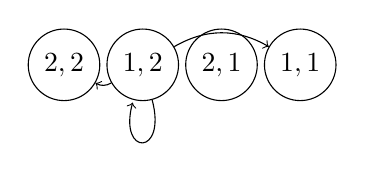
\begin{tikzpicture}[->,main/.style = {draw, circle}] 
			\node[main] (a) {$2, 2$}; 
			\node[main] (b) [right of=a] {$1, 2$};
			\node[main] (c) [right of=b] {$2, 1$};
			\node[main] (d) [right of=c] {$1, 1$};
			\path
			(b) edge[bend left, above] (a)
			    edge[loop below] (b)
				edge[bend left, above] (d);
		\end{tikzpicture}
		\caption{Markov Chain}
		\label{fig:s-exmp-2}
	\end{marginfigure}
For $n = 2$ and $m = 2$. Thus each $x_i$ can either be 1 or 2. Thus, \\
$T(x|x' = [1, 2]) = 0$ if $x = [2, 1]$ \\
$T(x|x' = [1,2]) = \frac{1}{2} P(x_1 = 1 | x_2 = 2) + \frac{1}{2} P(x_2 = 2 | x_1 = 1)$ if $x = [1,2]$ \\
$T(x|x' = [1,2]) = P(x_1 = 2 | x_2 = 2)$ if $x = [2, 2]$ \\
$T(x|x' = [1,2]) = P(x_2 = 2 | x_1 = 1)$ if $x = [1, 2]$  \\
For the above transition probabilities, we can have a graph as shown in Figure \ref{fig:s-exmp-2}. 
\end{exmp}
Consider finite state space $X$, where we have states $1$ to $m^n$ and say we choose an arbitrary initial state $x^0$ at $t = 0$. We want to calcualte $T(x | x^0)$. This $T(x|x^0)$ is a multinomial distribution over all states. We sample from this. At $t = 0$, $P_{t=0}(x) = 1$ if $x = x^0$ and $0$ else. At $t = 1$, we want $P_{t=1}(x) = T(x | x^0)$. At $t=2$, the probability of being in state $x$ is $P_{t=2}(x) = \sum_{x'} T(x | x') T(x' | x^0) = \sum_{x'} T(x|x') P_{t-1}(x')$. Thus in general
\begin{equation}
	P_t(x) = \sum_{x'} T(x|x') P_{t-1}(x')
\end{equation}
As $t \to \infty$, $P_{t+1}(x) \approx P_t(x)$ for convergence as $t\to\infty$ and this is equal to the stationary distribution $\pi(x)$. We are interested in $T(x|x')$ for which $P_{t+1}(x) = \sum_{x'} P_t(x') T(x|x')$ and as $t \to \infty$
\begin{equation}
	\pi(x) = \sum_{x'} \pi(x') T(x|x')
\end{equation}
has a unique solution for given $T(x|x')$ and $\pi(x)$ should be reachable from any initial state $x^0$ via Markov walks using $T(x|x')$.